\documentclass{beamer}

%\usepackage{lmodern}
\usepackage[font=scriptsize,skip=0pt,justification=justified,singlelinecheck=false]{caption}
%\usepackage{enumitem}
\usepackage{natbib}
\usepackage{bm}
\usepackage{mathtools}
\usepackage[makeroom]{cancel}


% Insert a Video
\usepackage{multimedia} 

% Using underline
\usepackage{soul}


%remove the icon
\setbeamertemplate{bibliography item}{}

%remove line breaks
\setbeamertemplate{bibliography entry title}{}
\setbeamertemplate{bibliography entry location}{}
\setbeamertemplate{bibliography entry note}{}
% Use number for caption
\setbeamertemplate{caption}[numbered]{}

\newtheorem{mydef}[theorem]{\Large \underline{\textbf{Definisi}}}

\makeatletter
\def\th@mystyle{%
    \normalfont % body font
    \setbeamercolor{block title example}{bg=blue,fg=white}
    \setbeamercolor{block body example}{bg=blue!20,fg=black}
    \def\inserttheoremblockenv{exampleblock}
  }
\makeatother
\theoremstyle{mystyle}
\newtheorem*{remark}{\textbf{Definition}}


% This file is a solution template for:

% - Talk at a conference/colloquium.
% - Talk length is about 20min.
% - Style is ornate.

% Copyright 2004 by Till Tantau <tantau@users.sourceforge.net>.
%
% In principle, this file can be redistributed and/or modified under
% the terms of the GNU Public License, version 2.
%
% However, this file is supposed to be a template to be modified
% for your own needs. For this reason, if you use this file as a
% template and not specifically distribute it as part of a another
% package/program, I grant the extra permission to freely copy and
% modify this file as you see fit and even to delete this copyright
% notice.  


\mode<presentation>
{
%  \usetheme{AnnArbor} % 
%	\usetheme{Frankfurt}
   \usetheme{Madrid}
%	\usetheme{Darmstadt}
  % or ...

%  \setbeamercovered{transparent}
  % or whatever (possibly just delete it)
}


\usepackage[english]{babel}
% or whatever

\usepackage[latin1]{inputenc}
% or whatever

\usepackage{times}
\usepackage[T1]{fontenc}
\usepackage{wasysym}

% Define absolute and norm
\DeclarePairedDelimiter\abs{\lvert}{\rvert}%
\DeclarePairedDelimiter\norm{\lVert}{\rVert}%

% ==============================
%       Redefine emphasize
% ==============================
\let\emph\relax % there's no \RedeclareTextFontCommand
\DeclareTextFontCommand{\emph}{\bfseries\em}


% Swap the definition of \abs* and \norm*, so that \abs
% and \norm resizes the size of the brackets, and the 
% starred version does not.
\makeatletter
\let\oldabs\abs
\def\abs{\@ifstar{\oldabs}{\oldabs*}}
%
\let\oldnorm\norm
\def\norm{\@ifstar{\oldnorm}{\oldnorm*}}
\makeatother

\usepackage{color}
\definecolor{myblue}{rgb}{.8,.8,1}
\usepackage{empheq}
% Or whatever. Note that the encoding and the font should match. If T1
% does not look nice, try deleting the line with the fontenc.

\newlength\mytemplen
\newsavebox\mytempbox

\makeatletter
\newcommand\mybluebox{%
    \@ifnextchar[%]
       {\@mybluebox}%
       {\@mybluebox[0pt]}}

\def\@mybluebox[#1]{%
    \@ifnextchar[%]
       {\@@mybluebox[#1]}%
       {\@@mybluebox[#1][0pt]}}

\def\@@mybluebox[#1][#2]#3{
    \sbox\mytempbox{#3}%
    \mytemplen\ht\mytempbox
    \advance\mytemplen #1\relax
    \ht\mytempbox\mytemplen
    \mytemplen\dp\mytempbox
    \advance\mytemplen #2\relax
    \dp\mytempbox\mytemplen
    \colorbox{myblue}{\hspace{1em}\usebox{\mytempbox}\hspace{1em}}}

\makeatother

\title[Pentingnya Kepribadian Dalam Pernikahan] % (optional, use only with long paper titles)
{\textbf{Pentingnya Kepribadian Dalam Pernikahan}}

%\subtitle
%{\textit{Perbedaan Pria dan Wanita}}

\author[Hendra Bunyamin] % (optional, use only with lots of authors)
{Hendra Bunyamin}
%{F.~Author\inst{1} \and S.~Another\inst{2}} --> original
% - Give the names in the same order as the appear in the paper.
% - Use the \inst{?} command only if the authors have different
%   affiliation.

\institute[ ] % (optional, but mostly needed)
{
%  \inst{1}%
  \hfill \break
  \hfill \break 
  \hfill \break
  \hfill \break
  \large
  Bimbingan Pranikah\\
  GKI Anugerah
%  \and
%  \inst{2}%
%  Department of Theoretical Philosophy\\
%  University of Elsewhere
}
% - Use the \inst command only if there are several affiliations.
% - Keep it simple, no one is interested in your street address.

%\date[CFP 2003] % (optional, should be abbreviation of conference name)
%{Conference on Fabulous Presentations, 2003}
% - Either use conference name or its abbreviation.
% - Not really informative to the audience, more for people (including
%   yourself) who are reading the slides online

\subject{PowerPoint}
% This is only inserted into the PDF information catalog. Can be left
% out. 

% If you have a file called "university-logo-filename.xxx", where xxx
% is a graphic format that can be processed by latex or pdflatex,
% resp., then you can add a logo as follows:

\pgfdeclareimage[height=1.2cm]{university-logo}{images/logo-gkia-komit}
\logo{\pgfuseimage{university-logo}}


% Delete this, if you do not want the table of contents to pop up at
% the beginning of each subsection:
\AtBeginSection[]
{
  \begin{frame}<beamer>{Outline}
    \tableofcontents[currentsection,currentsection]
  \end{frame}
}


% If you wish to uncover everything in a step-wise fashion, uncomment
% the following command: 

%\beamerdefaultoverlayspecification{<+->}

\begin{document}

\begin{frame}
  \titlepage
\end{frame}

\begin{frame}{The Bunyamins}
	\centering
	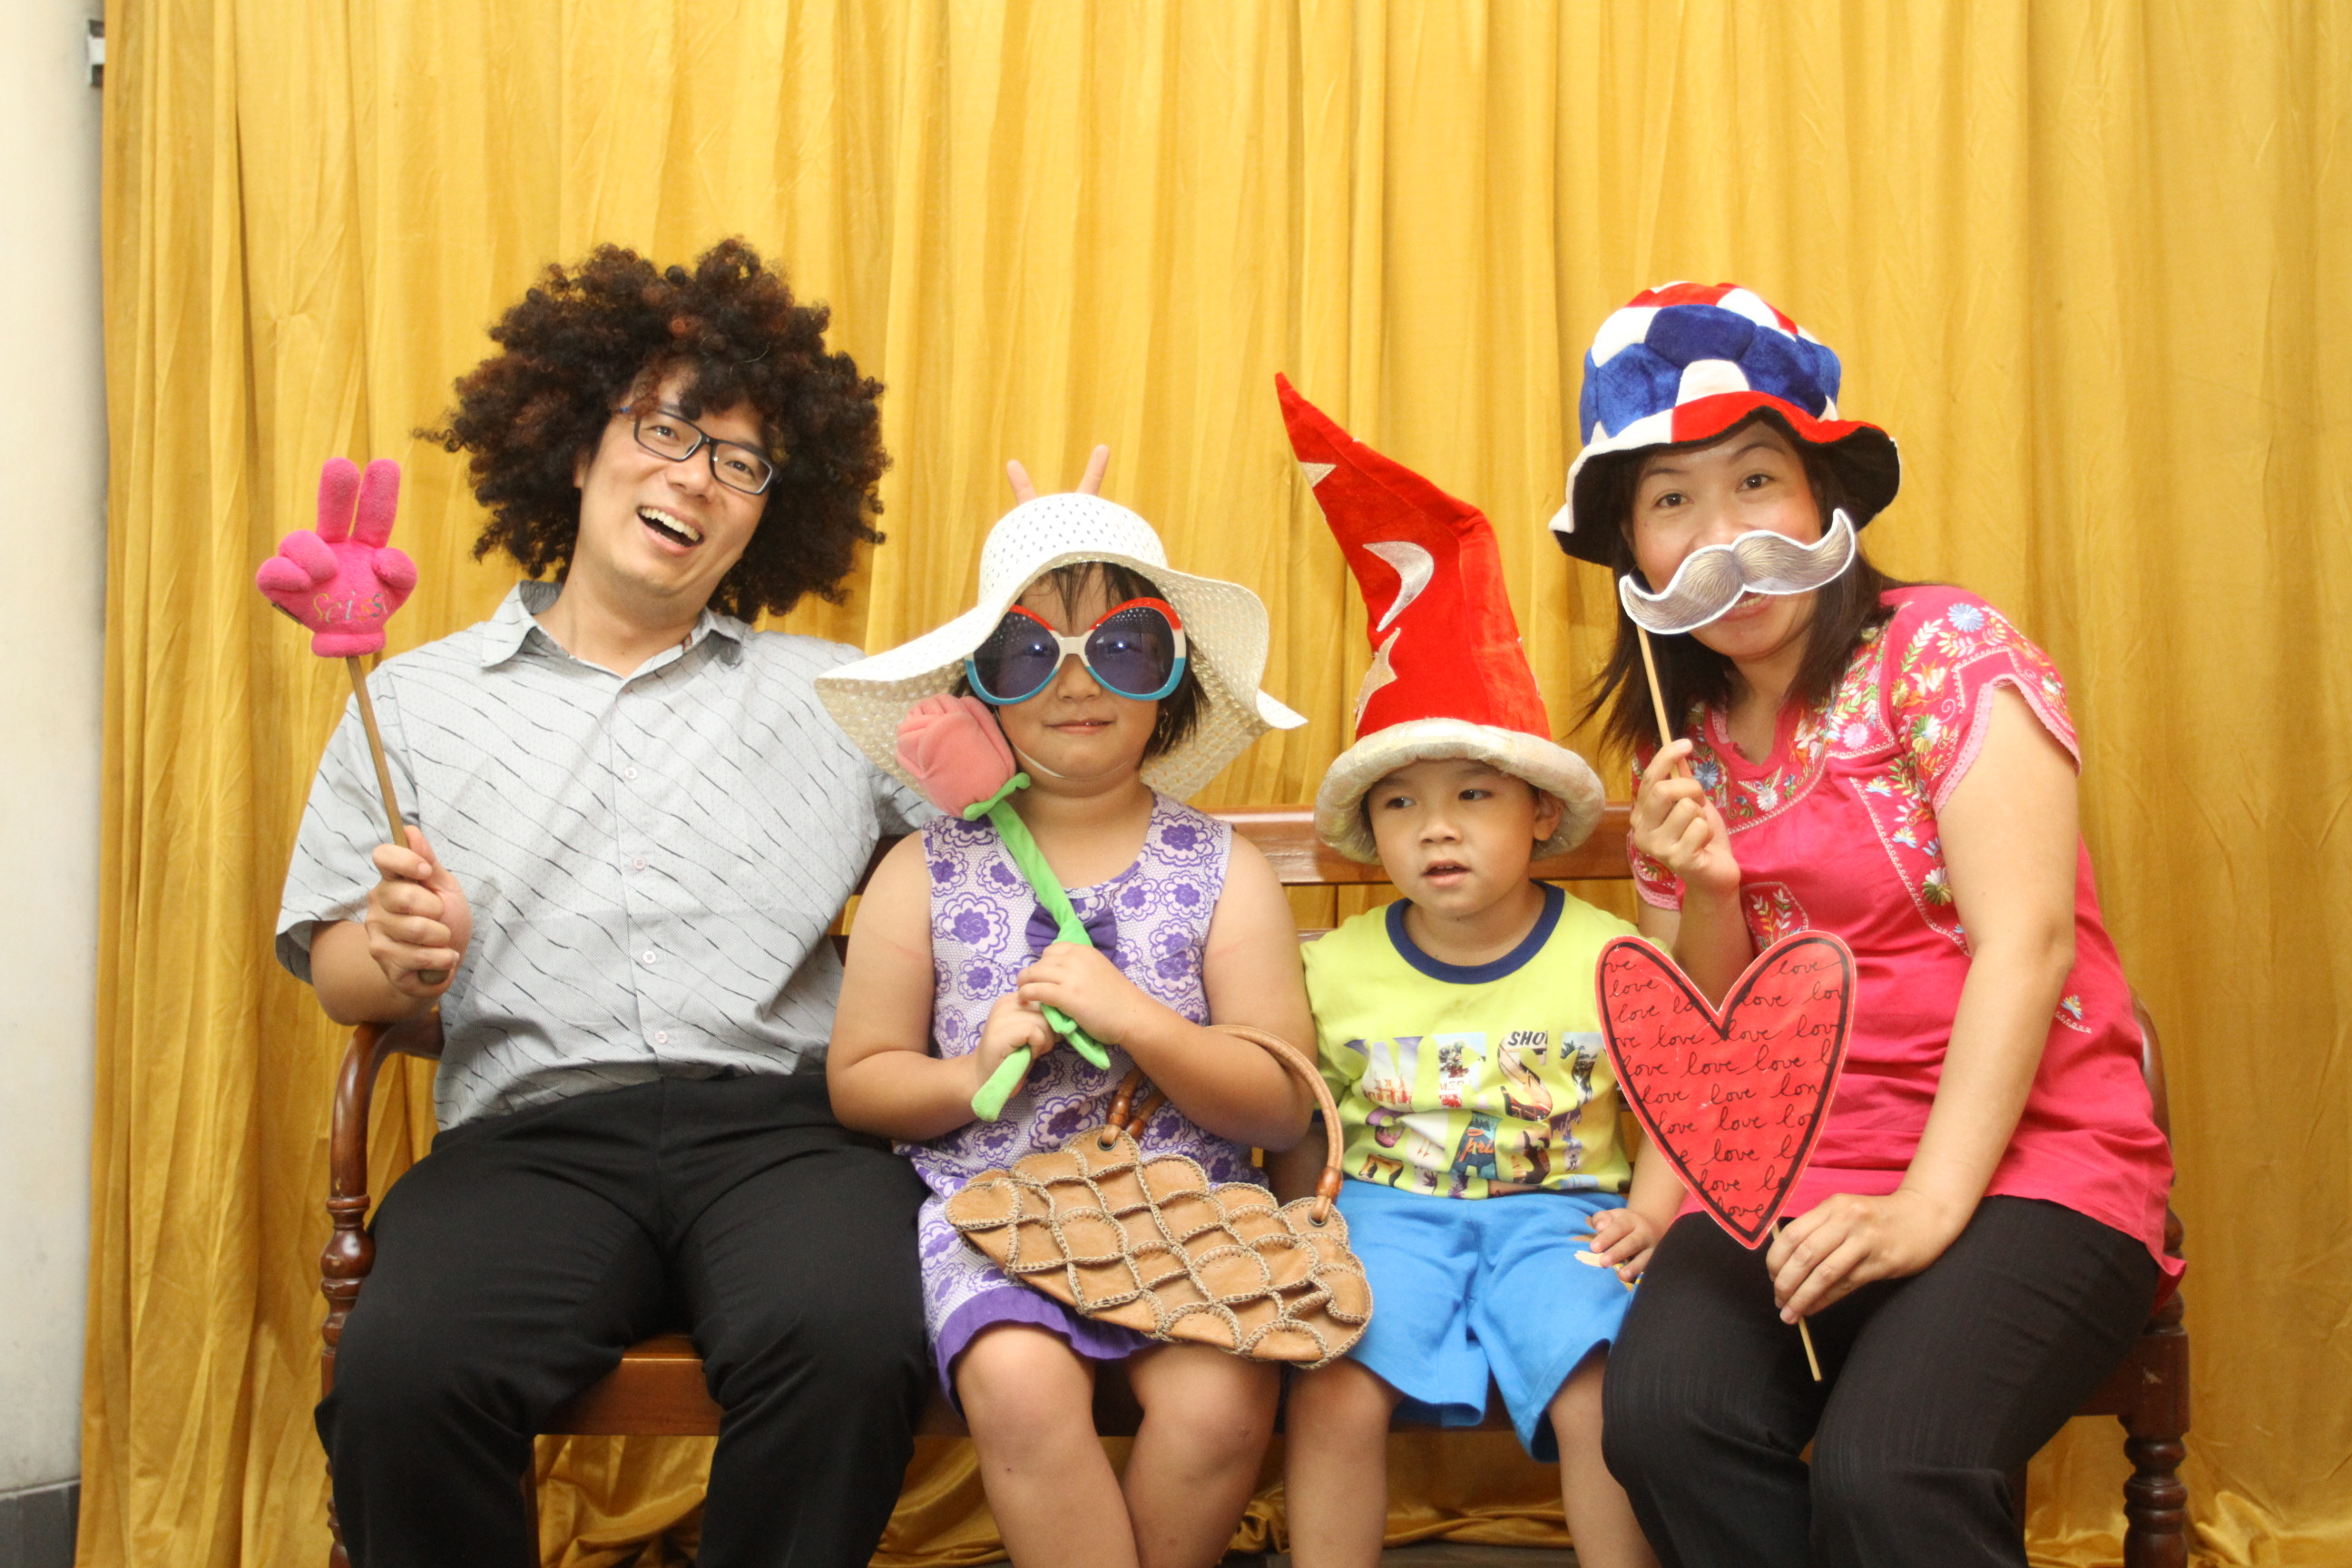
\includegraphics[scale=.125]{images/family-gullit}
\end{frame}

\begin{frame}{Outline}
  \tableofcontents
  % You might wish to add the option [pausesections]
\end{frame}


% Structuring a talk is a difficult task and the following structure
% may not be suitable. Here are some rules that apply for this
% solution: 

% - Exactly two or three sections (other than the summary).
% - At *most* three subsections per section.
% - Talk about 30s to 2min per frame. So there should be between about
%   15 and 30 frames, all told.

% - A conference audience is likely to know very little of what you
%   are going to talk about. So *simplify*!
% - In a 20min talk, getting the main ideas across is hard
%   enough. Leave out details, even if it means being less precise than
%   you think necessary.
% - If you omit details that are vital to the proof/implementation,
%   just say so once. Everybody will be happy with that.

%\begin{frame}{Make Titles Informative. Use Uppercase Letters.}{Subtitles are optional.}


\section{Tujuan Sharing Hari Ini}
\begin{frame}{Tujuan Sharing Hari Ini \citep{susabda2021konseling}}
	\begin{itemize}
		\item<2-> Menolong pasangan menyadari bahwa \textit{kebahagiaan} dan \textit{keberhasilan pernikahan} sangat ditentukan oleh unsur \textit{kepribadian}.
		
		\bigskip
		\item<3-> \textit{Menolong pasangan} menyadari perlunya menyusun \textit{strategi yang tepat} untuk menyelesaikan masalah-masalah kepribadian.
	\end{itemize}
\end{frame}

\section{Keberhasilan Pernikahan Ditentukan oleh Kepribadian}
\begin{frame}{Keberhasilan Pernikahan Ditentukan Kepribadian} 
	\begin{itemize}
		\item<2-> Alkitab mencatat berulang kali adanya pasangan anak-anak Tuhan yang saling mencintai dan beriman teguh tetapi mengalami persoalan-persoalan yang seharusnya tidak perlu karena kelemahan masing-masing: \textbf{Kejadian 20:1-18}.
		\item<3-> Dampaknya, Abraham \& Sara menghadapi kesulitan yang penyelesaiannya tidak mudah dan cukup kompleks.
		\item<4-> Jadi pasangan yang beriman teguh dan saling mencintai \textit{tidak dengan sendirinya terbebas} dari bahaya yang mengancam keutuhan kehidupan pernikahan mereka.		   
	\end{itemize}
\end{frame}

\begin{frame}{Anak Belajar dari Kehidupan (by D. L. Nolte)}
	\onslide<2->{Jika anak dibesarkan dengan \textbf{celaan}, ia belajar \textbf{memaki}.} \\ 
	\onslide<3->{Jika anak dibesarkan dengan \textbf{permusuhan}, ia belajar \textbf{berkelahi}.} \\
	\onslide<4->{Jika anak dibesarkan dengan \textbf{cemoohan}, ia belajar \textbf{rendah diri}.} \\ 
	\onslide<5->{Jika anak dibesarkan dengan \textbf{penghinaan}, ia belajar \textbf{menghina diri sendiri}.} \\
	\onslide<6->{Jika anak dibesarkan dengan \textbf{toleransi}, ia belajar \textbf{menahan diri}.} \\
	\onslide<7->{Jika anak dibesarkan dengan \textbf{pujian}, ia belajar \textbf{menghargai}.} \\
	\onslide<8->{Jika anak dibesarkan dengan \textbf{perlakuan yang baik}, ia belajar \textbf{keadilan}.} \\
	\onslide<9->{Jika anak dibesarkan dengan \textbf{rasa aman}, ia belajar \textbf{menaruh kepercayaan}.} \\ 
	\onslide<10->{Jika anak dibesarkan dengan \textbf{dukungan}, ia belajar \textbf{menghargai diri}.} \\
	\onslide<11->{Jika anak dibesarkan \textbf{kasih sayang} dan \textbf{persahabatan}, ia belajar \textbf{menemukan cinta dalam kehidupan}.}
\end{frame}

\begin{frame}{Pengalaman Masa Kecil Anda Sendiri (1/3)}
	\begin{itemize}
		\item<2-> Mungkin anda pernah mengalami pengalaman dengan orang tua yang melukai dan menyakitkan.
		\item<3-> Mungkin anda dibesarkan dalam keluarga kurang harmonis atau mungkin juga pengalaman-pengalaman masa kecil anda sudah terlupakan tetapi \textit{dampaknya membekas dan membentuk kepribadian anda sekarang}.
	\end{itemize}
\end{frame}


\begin{frame}{Pengalaman Masa Kecil Anda Sendiri (2/3)}
	Sebagai contoh:
	\begin{itemize}
		\item<2-> Kecenderungan anda untuk selalu memaksakan kehendak.
		\item<3-> Kebiasaan anda untuk tidak menepati janji dan tidak pernah minta maaf.
		\item<4-> Kecenderungan anda untuk memanipulasi semata-mata untuk kepentingan anda sendiri.
		\item<5-> Kebiasaan anda yang kekanak-kanakan pada saat anda dikecewakan oleh pasangan misalnya tiba-tiba anda meninggalkan pasangan tanpa pamit, ngambek, ancam bunuh diri, dan menghukum dengan tidak berkomunikasi selama berhari-hari.
	\end{itemize}
\end{frame}


\begin{frame}{Pengalaman Masa Kecil Anda Sendiri (3/3)}
	Sebagai contoh:
	\begin{itemize}
		\item<2-> Kecenderungan anda untuk selalu tergantung pada orang tua, misal ketergantungan finansial, pengambilan keputusan dalam hal yang sederhana.
		\item<3-> Kecenderungan anda menghindari konflik karena takut menghadapi realitas misalnya perbedaan pendapat, atau hal-hal yang memberikan beban tanggung jawab yang lebih besar.
	\end{itemize}
\end{frame}

\begin{frame}{Menolong Pasangan ttg Masalah Kepribadian}
	\begin{itemize}
		\item<2-> Masalah kepribadian merupakan salah satu aspek yang \textit{paling sulit diatasi}.
		\item<3-> Kadang-kadang untuk masalah kepribadian diperlukan bantuan \textit{konselor} dan \textit{terapis yang profesional}, khususnya jikalau akibat masalah tersebut sudah melumpuhkan banyak fungsi dari pernikahan yang akan dibentuk. 
		\item<4-> Meskipun demikian, sesuai dengan tanggung jawab kristiani, setiap individu yang siap menikah, seharusnya \textbf{belajar menemukan strategi untuk menyelesaikan masalah-masalah kepribadiannya sendiri}.
	\end{itemize}
\end{frame}

\section{Strategi Menyelesaikan Masalah Kepribadian}
\begin{frame}{Strategi Menyelesaikan Masalah Kepribadian (1/3)}
	\onslide<2->{\textbf{Keterbukaan dan kejujuran}}
	\begin{itemize}
		\item<3-> Keberanian individu untuk belajar terbuka dan jujur baik dengan dirinya sendiri maupun dengan pasangannya.
		\item<4-> Sistem komunikasi dialogis $\Rightarrow$ mencoba menghadirkan dirinya secara \textit{utuh} di hadapan pasangannya. 
		\item<5-> Mengkomunikasikan keutuhan pribadi, misalnya dalam menghadapi pengalaman yang tidak adil, juga dapat memberikan alasan mengapa ia marah dan frustasi.
		\item<6-> Dengan komunikasi yang terbuka dan jujur, makin lama individu makin mengenal dirinya sendiri dan ia makin dikenal oleh pasangannya sehingga upaya-upaya perbaikan akan lebih terbuka bagi mereka.   
	\end{itemize}
\end{frame}

\begin{frame}{Strategi Menyelesaikan Masalah Kepribadian (2/3)}
	\onslide<2->{\textbf{Berani beresiko dalam memasuki proses perbaikan}}
	\begin{itemize}
		\item<3-> Dengan terciptanya komunikasi yang semakin dialogis, akan muncul banyak kemungkinan keterkiliran dan konflik. 
		\item<4-> Mengapa demikian? \onslide<5->{Individu dengan kelemahan kepribadian sering kali merasa diobjekkan, seolah-olah dirinya sendiri yang harus berubah sehingga secara otomatis jiwanya akan memakai mekanisme pertahanan diri.}
		\begin{itemize}
			\item<6-> \textit{Forgetting} $\Rightarrow$ melupakan dan tidak mau dilanjutkan,
			\item<7-> \textit{Projection} $\Rightarrow$ memindahkan kesalahan pada orang tua yang sudah membesarkan dirinya, atau
			\item<8-> Rasionalisasi $\Rightarrow$ membahas kelemahan tanpa melibatkan dirinya secara utuh.  
		\end{itemize}
	\end{itemize}
\end{frame}


\begin{frame}{Strategi Menyelesaikan Masalah Kepribadian (3/3)}
	\textbf{Berani beresiko dalam memasuki proses perbaikan}
	\begin{itemize}
		\item<2-> Bagi pasangannya, proses penyelesaian masalah kepribadian bisa sangat melelahkan karena biasanya harus melalui proses yang panjang. 
		\item<3-> Ketidaksabaran dan kesulitan menerima realitas kelemahan seringkali merupakan kendala yang utama. 
		\item<4-> Sebagai pasangan, ia bisa berulang kali kehilangan pengharapan sehingga tergoda untuk memaksakan perubahan sesuai dengan waktu yang dikehendakinya sendiri. 
		\item<5-> Sebagai contoh: menghadapi calon istri yang naif dan kekanak-kanakkan, dia bisa menjadi sangat kejam misalnya, tega membiarkan pasangannya pulang dari kerja lembur sendiri, padahal dulu ia biasa menjemput.
	\end{itemize}
\end{frame}

% \textcolor <6-> {orange} {\textbf<6->{Supervised Learning}}

\section{The Major Personality Models}
\begin{frame}{The Major Personality Models}
	There are many personality models, but four of the most popular \citep{crystal2015guide} are 
	\begin{itemize}
		\item<2-> \textcolor <6-> {orange} {\textbf<6->{DISC}},    
		\item<3-> 16 Personalities, 
		\item<4-> Enneagram, and 
		\item<5-> Big Five.  
	\end{itemize}	
\end{frame}

\begin{frame}{DISC}
	\begin{itemize}
		\item<2-> DISC is a "four-factor" personality model, meaning that it groups people into four categories based on behavior patterns.
		\item<3-> Each category consists of a set of personality traits. 
		\item<4-> Everyone has a primary category, and often a second category.
		\item<5-> DISC was developed in the early 1900s by psychologist William Marston, the same man who also happened to create \textit{Wonder Woman} and the \textit{polygraph}. 
		\item<6-> It resembles other four-factor models that have been around for more than 2,000 years, when Hippocrates first described the "four temperaments". 
	\end{itemize}
\end{frame}

\begin{frame}{D = Dominance}
	\begin{center}
		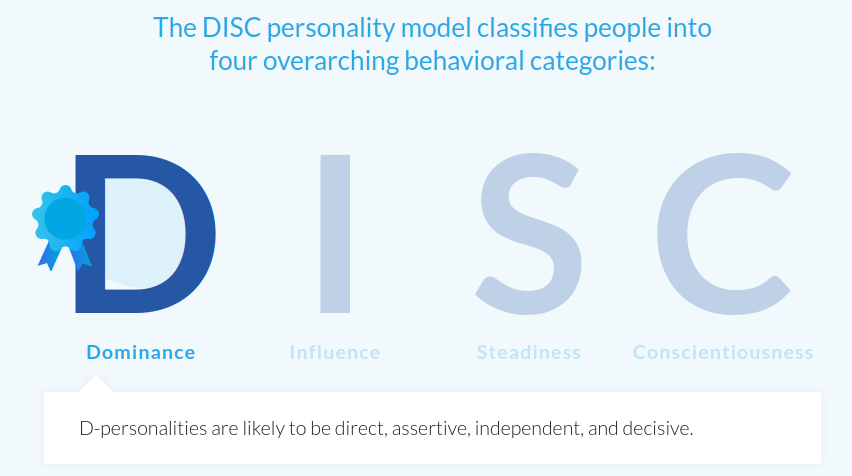
\includegraphics[scale=.35]{images/d-of-disc}
	\end{center}
\end{frame}

\begin{frame}{I = Influence}
	\begin{center}
		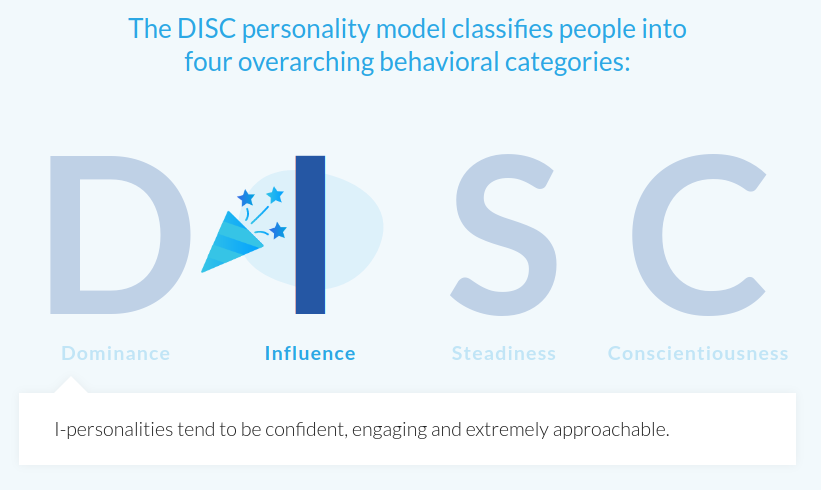
\includegraphics[scale=.35]{images/i-of-disc}
	\end{center}
\end{frame}

\begin{frame}{S = Steadiness}
	\begin{center}
		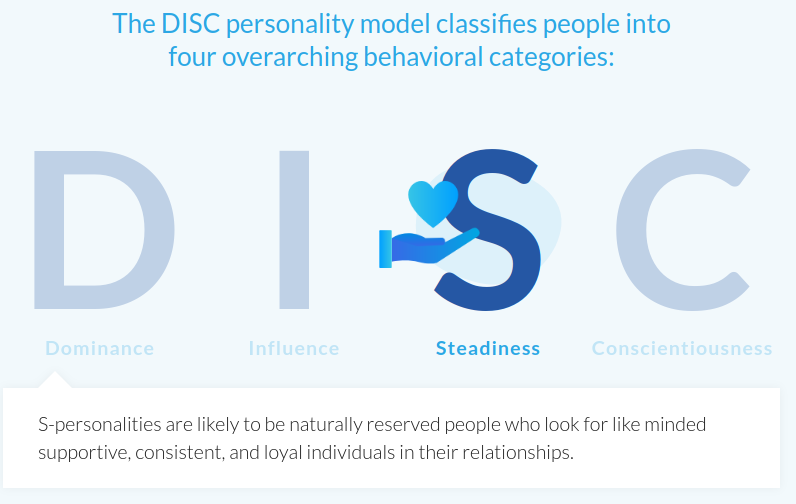
\includegraphics[scale=.35]{images/s-of-disc}
	\end{center}
\end{frame}

\begin{frame}{C = Conscientiousness}
	\begin{center}
		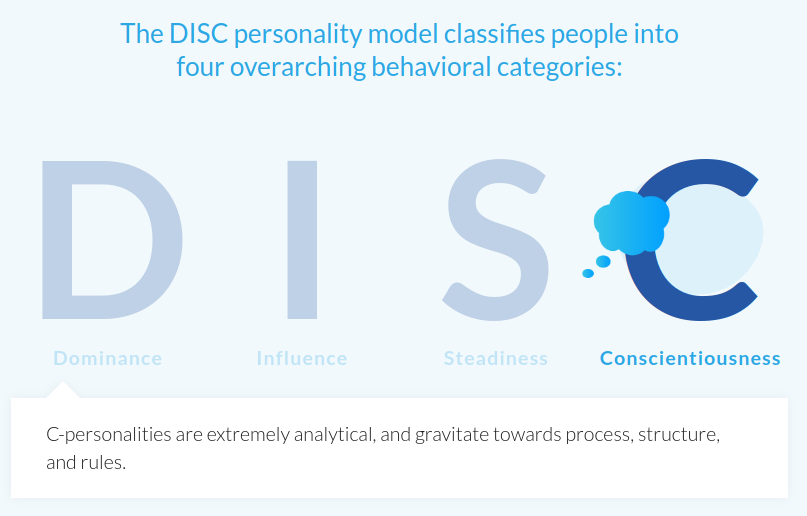
\includegraphics[scale=.35]{images/c-of-disc}
	\end{center}
\end{frame}

\begin{frame}{Why use the DISC test?}
	Because it teaches \textbf{empathy}. 
	\begin{itemize}
		\item<2-> The DISC assessment is the best resource for an individual to understand how to cater their behavior to the situation. 
		\item<3-> That's why we use DISC over other like-minded tests such as Myers-Briggs, The Color Code, or the myriad of options available.
	\end{itemize}
\end{frame}


\begin{frame}{DISC Types (1/2)}
	\begin{center}
		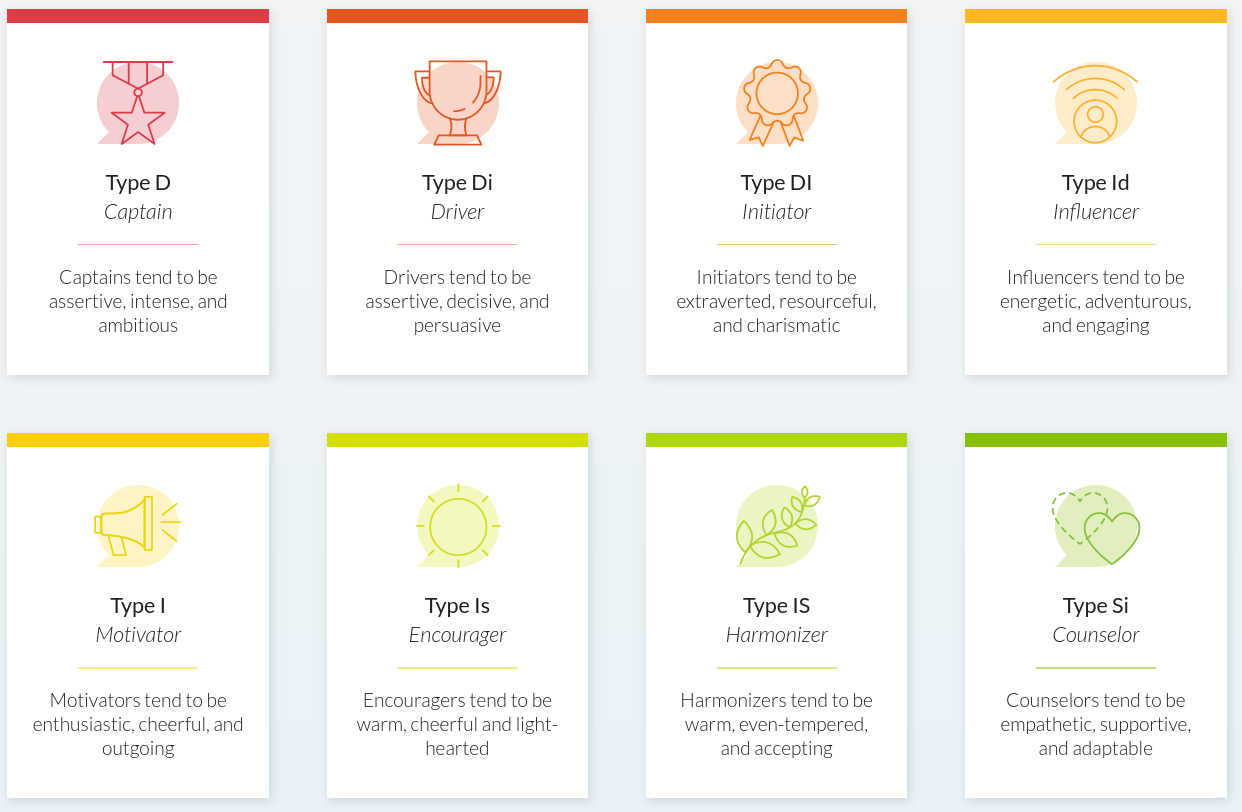
\includegraphics[scale=.25]{images/complete-disc-1}
	\end{center}
\end{frame}

\begin{frame}{DISC Types (2/2)}
	\begin{center}
		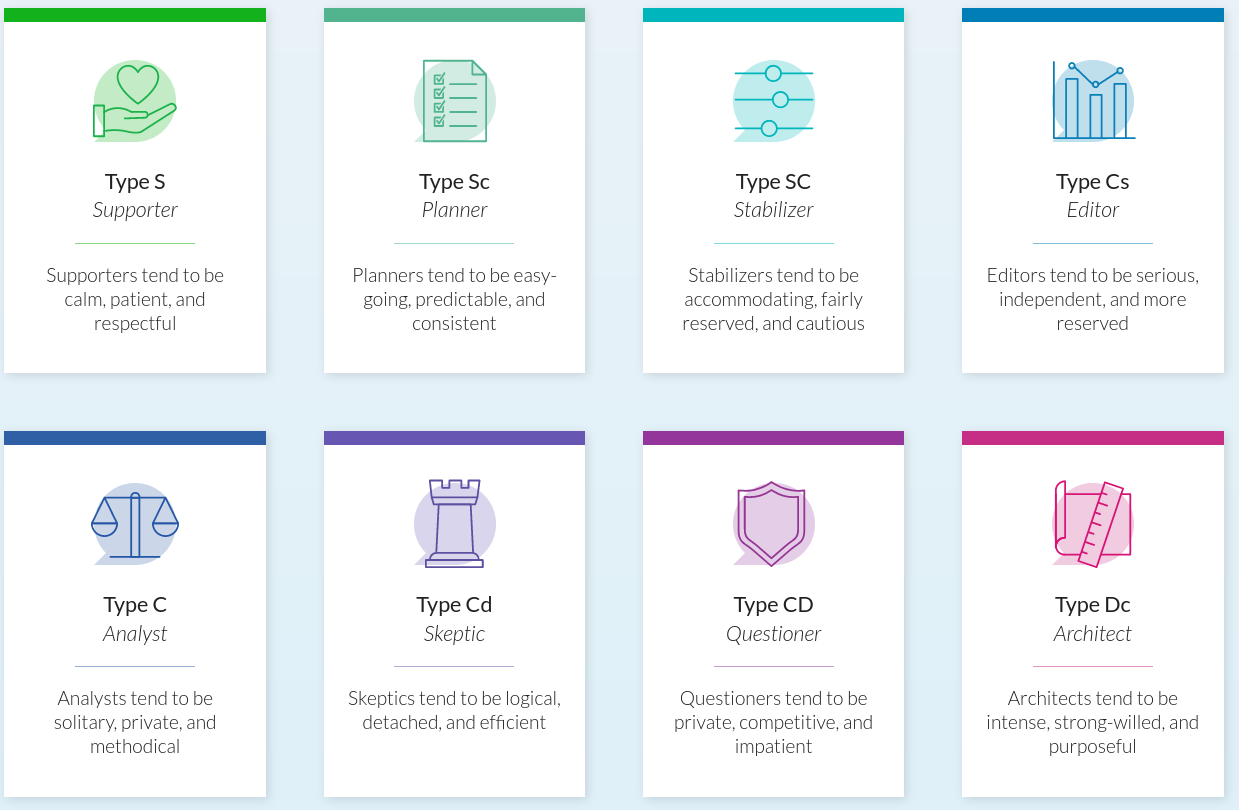
\includegraphics[scale=.25]{images/complete-disc-2}
	\end{center}
\end{frame}

\begin{frame}{Link untuk DISC Personality Test}
	\begin{itemize}
		\item<2-> Link untuk DISC Personality Test: \textbf{\url{https://www.crystalknows.com/app/assessment}}
		
		\bigskip
 		\item<3-> List semua tipe DISC: \textbf{\url{https://www.crystalknows.com/disc/types}} 
		
		\bigskip
		\item<4-> Contoh satu tipe DISC, \textbf{Sc} (\textit{Planner}): \\
		\textbf{\url{https://www.crystalknows.com/disc/sc-personality-type}} 
	\end{itemize}
\end{frame}

\section{The DISC Types}
\begin{frame}{Tipe D: Captain}
	\begin{center}
		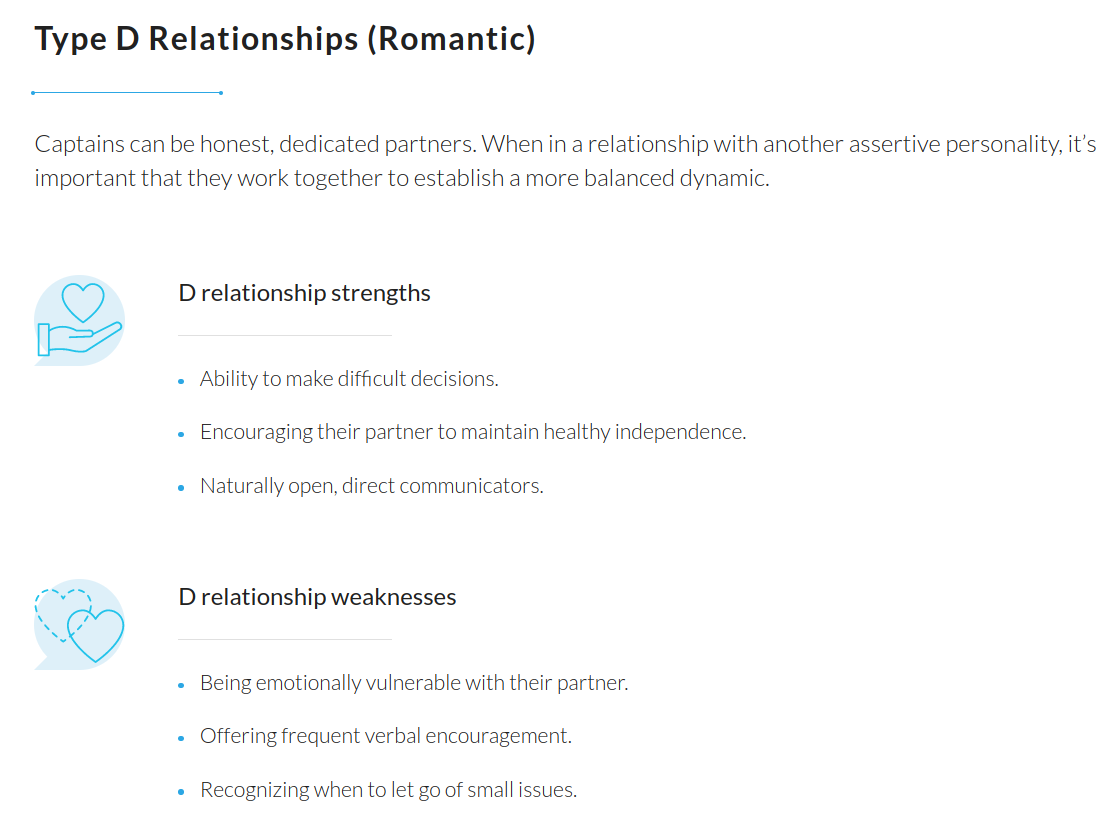
\includegraphics[scale=.275]{images/d}
	\end{center}
\end{frame}

\begin{frame}{Tipe Di: Driver}
	\begin{center}
		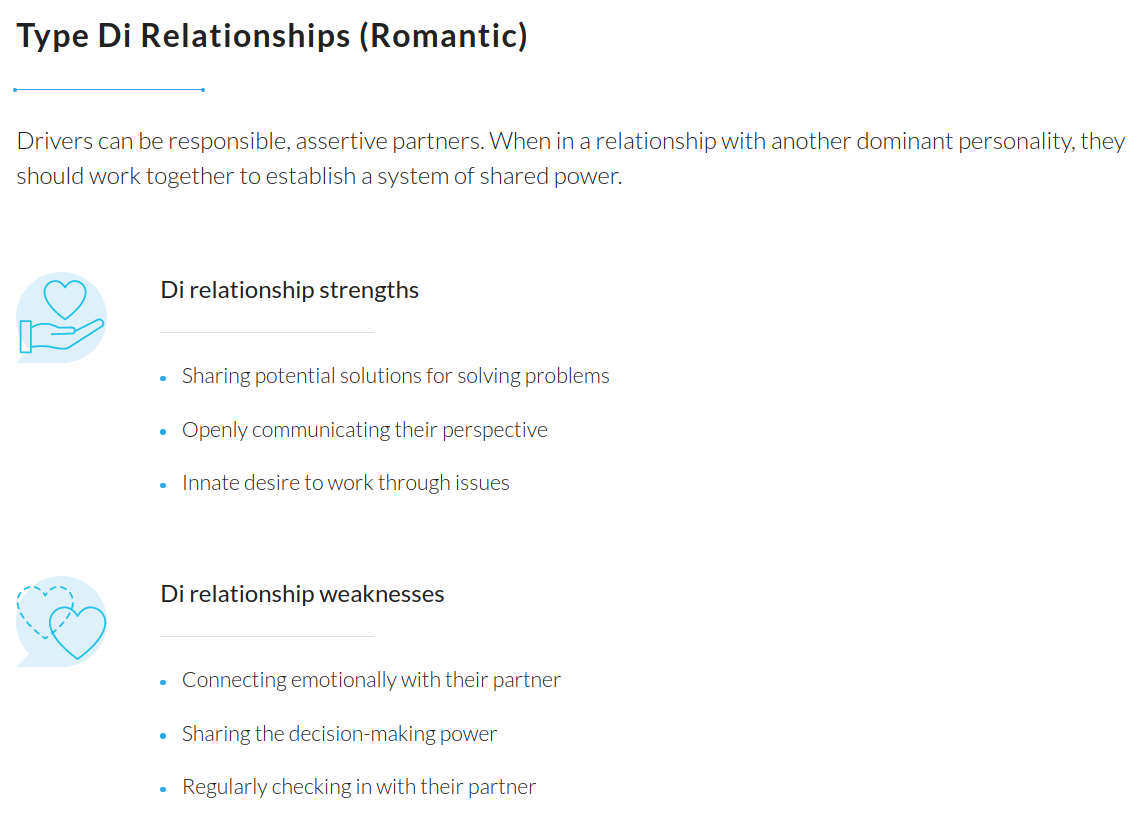
\includegraphics[scale=.275]{images/di}
	\end{center}
\end{frame}

\begin{frame}{Tipe DI: Initiator}
	\begin{center}
		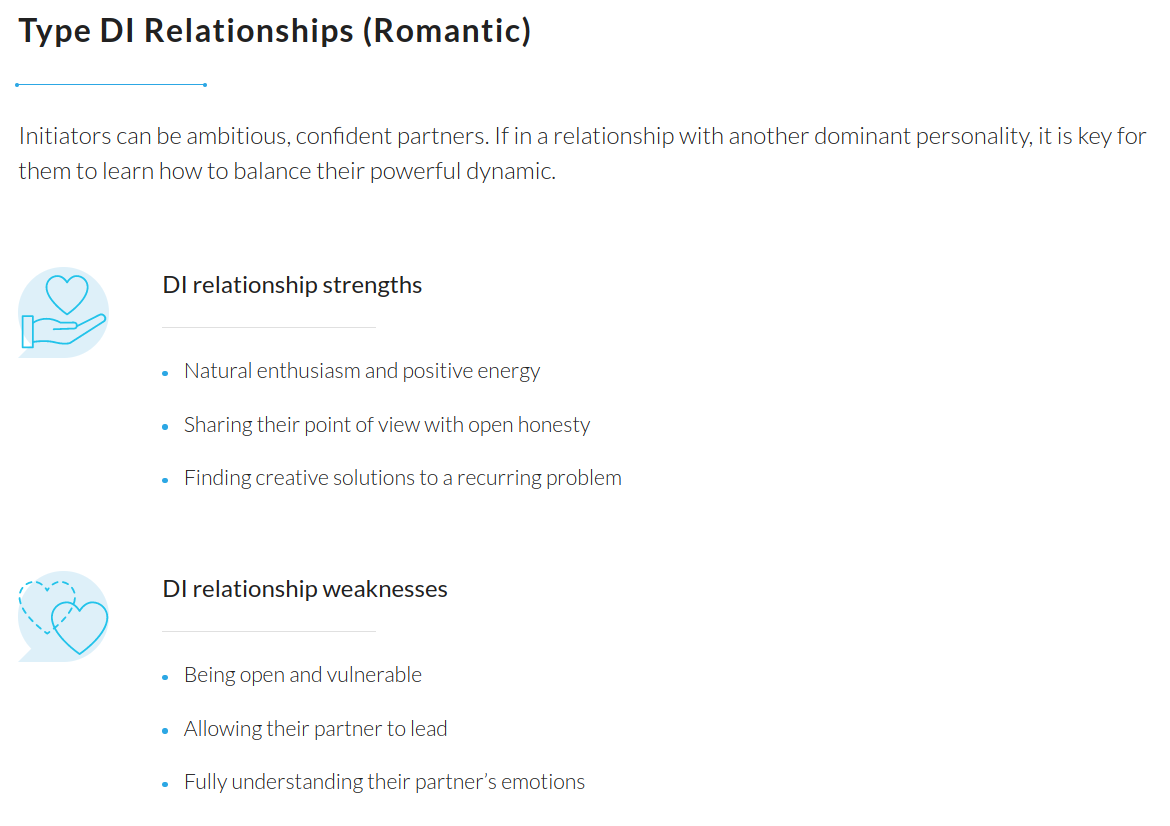
\includegraphics[scale=.275]{images/DI}
	\end{center}
\end{frame}

\begin{frame}{Tipe Id: Influencer}
	\begin{center}
		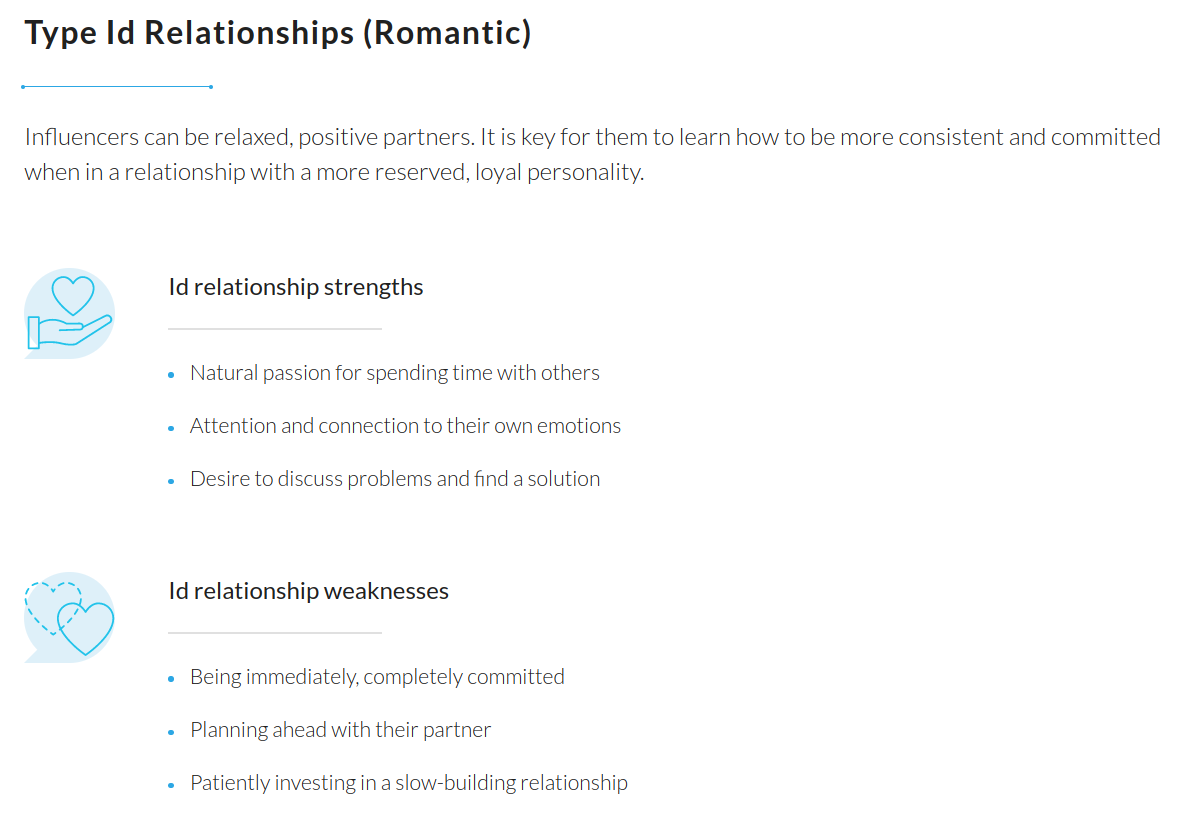
\includegraphics[scale=.275]{images/Id}
	\end{center}
\end{frame}

\begin{frame}{Tipe I: Motivator}
	\begin{center}
		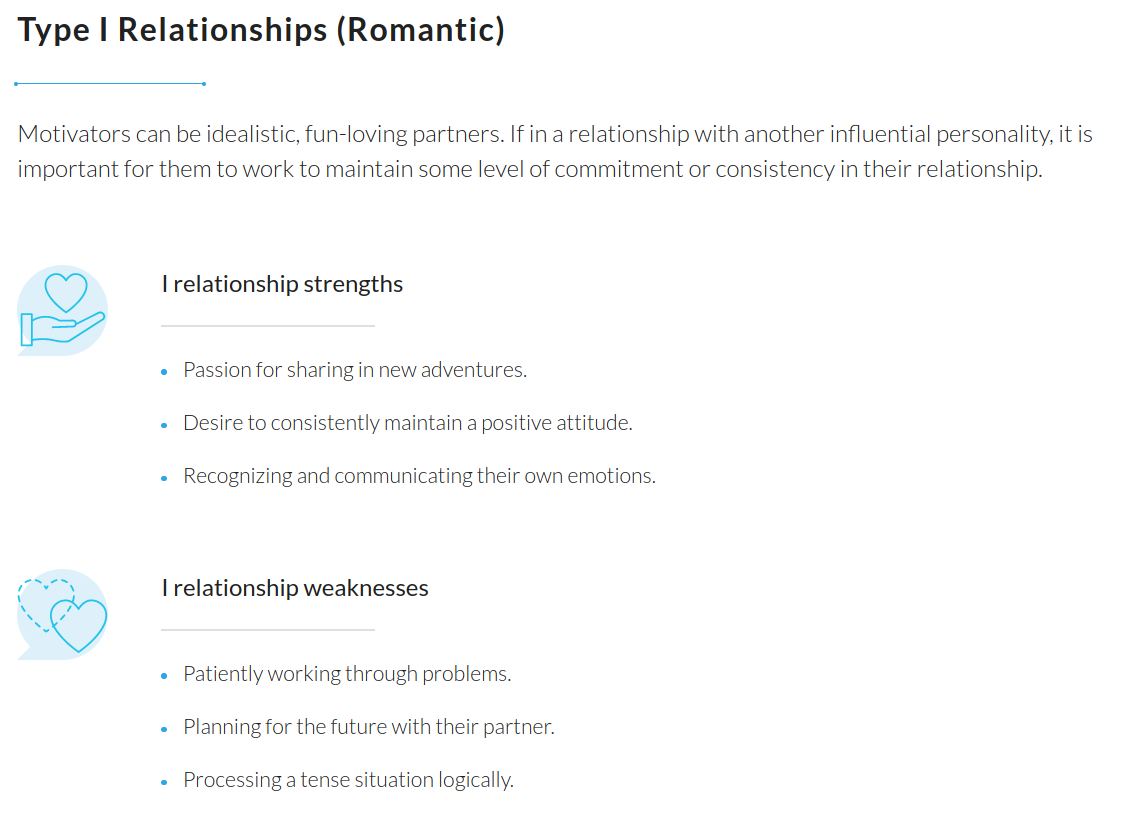
\includegraphics[scale=.275]{images/I}
	\end{center}
\end{frame}

\begin{frame}{Tipe Is: Encourager}
	\begin{center}
		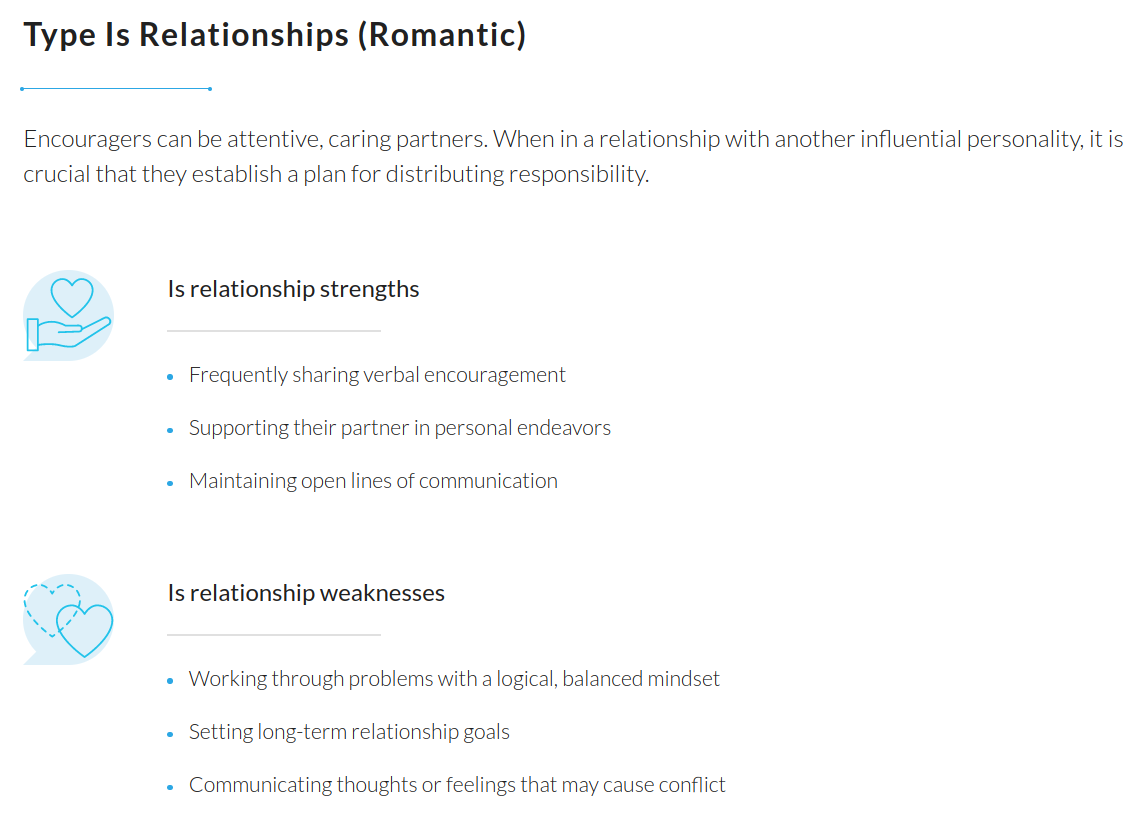
\includegraphics[scale=.275]{images/Is}
	\end{center}
\end{frame}

\begin{frame}{Tipe IS: Harmonizer}
	\begin{center}
		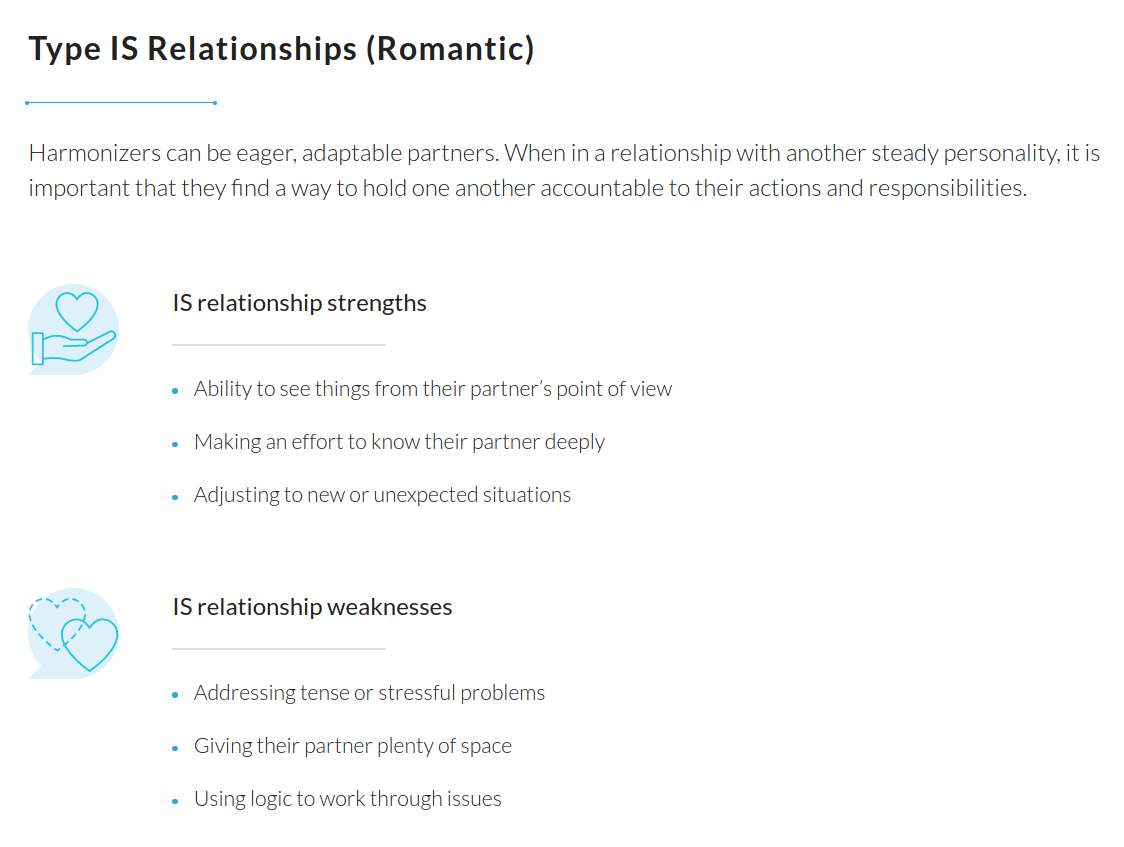
\includegraphics[scale=.275]{images/IS}
	\end{center}
\end{frame}

\begin{frame}{Tipe Si: Counselor}
	\begin{center}
		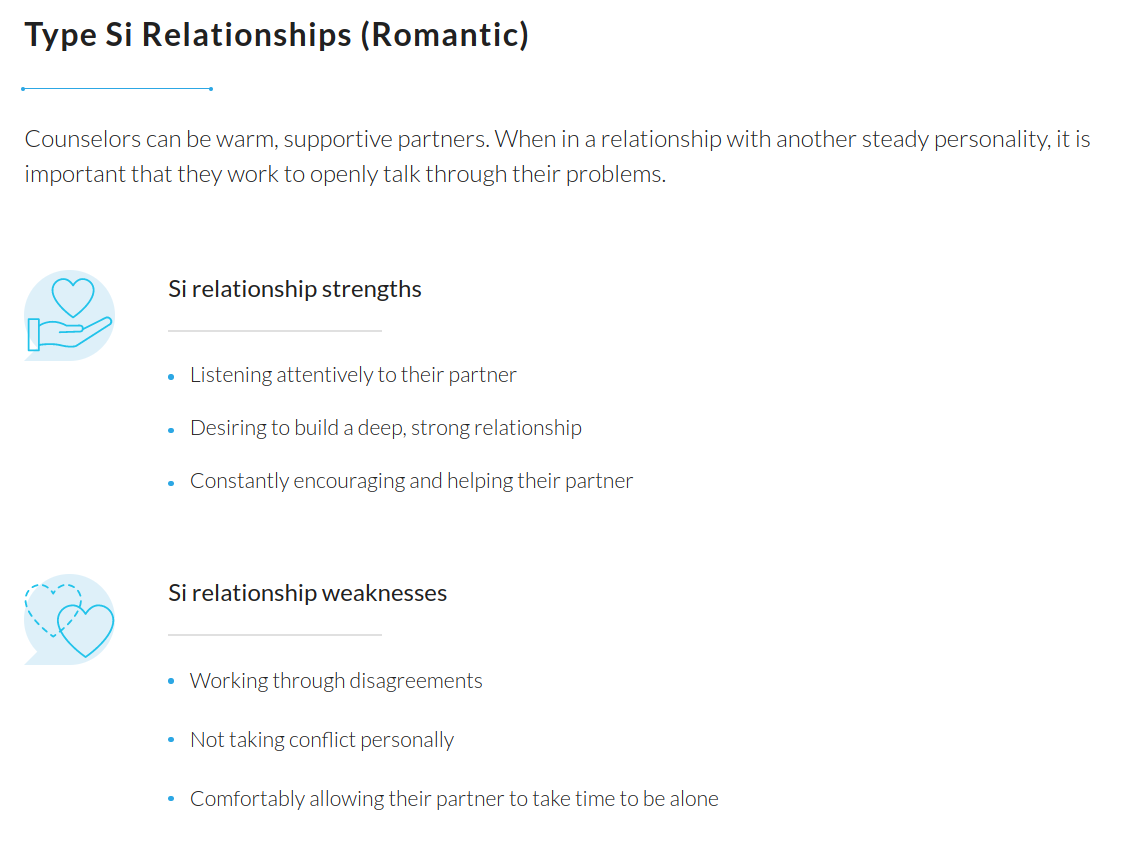
\includegraphics[scale=.275]{images/Si}
	\end{center}
\end{frame}

\begin{frame}{Tipe S: Supporter}
	\begin{center}
		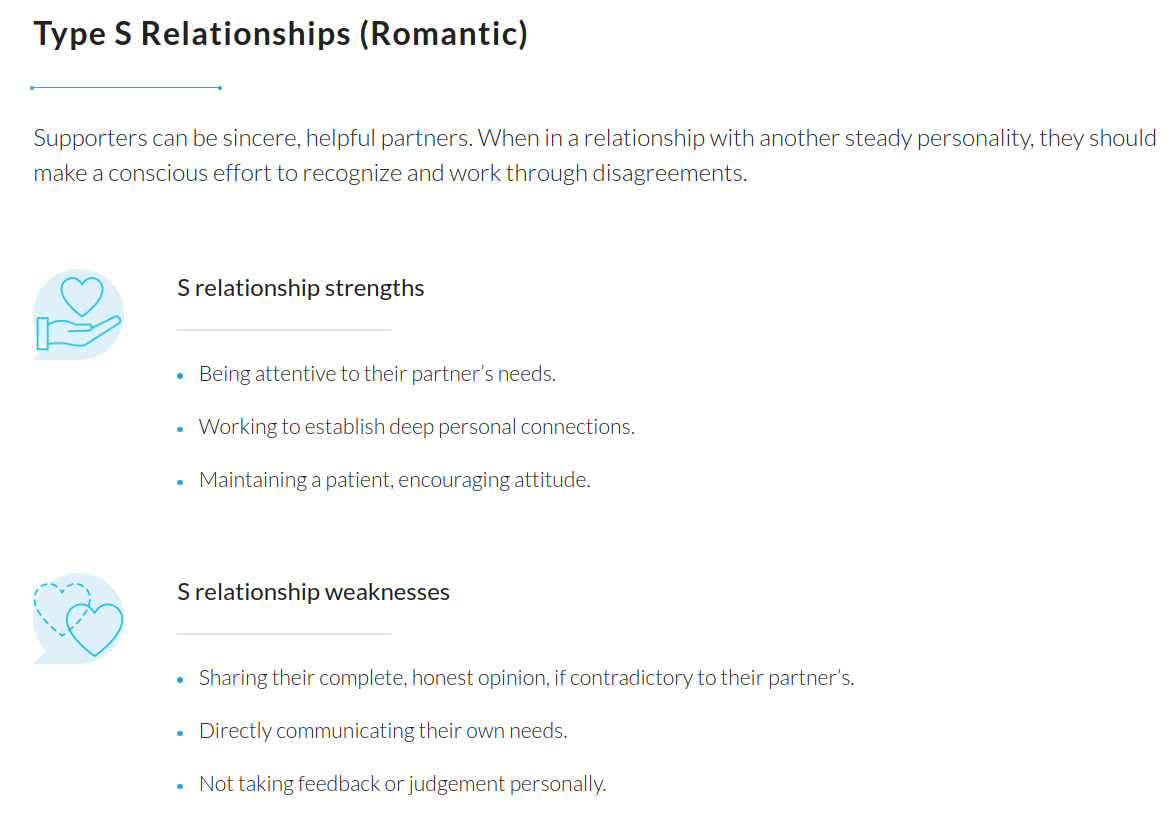
\includegraphics[scale=.275]{images/S}
	\end{center}
\end{frame}


\begin{frame}{Tipe Sc: Planner}
	\begin{center}
		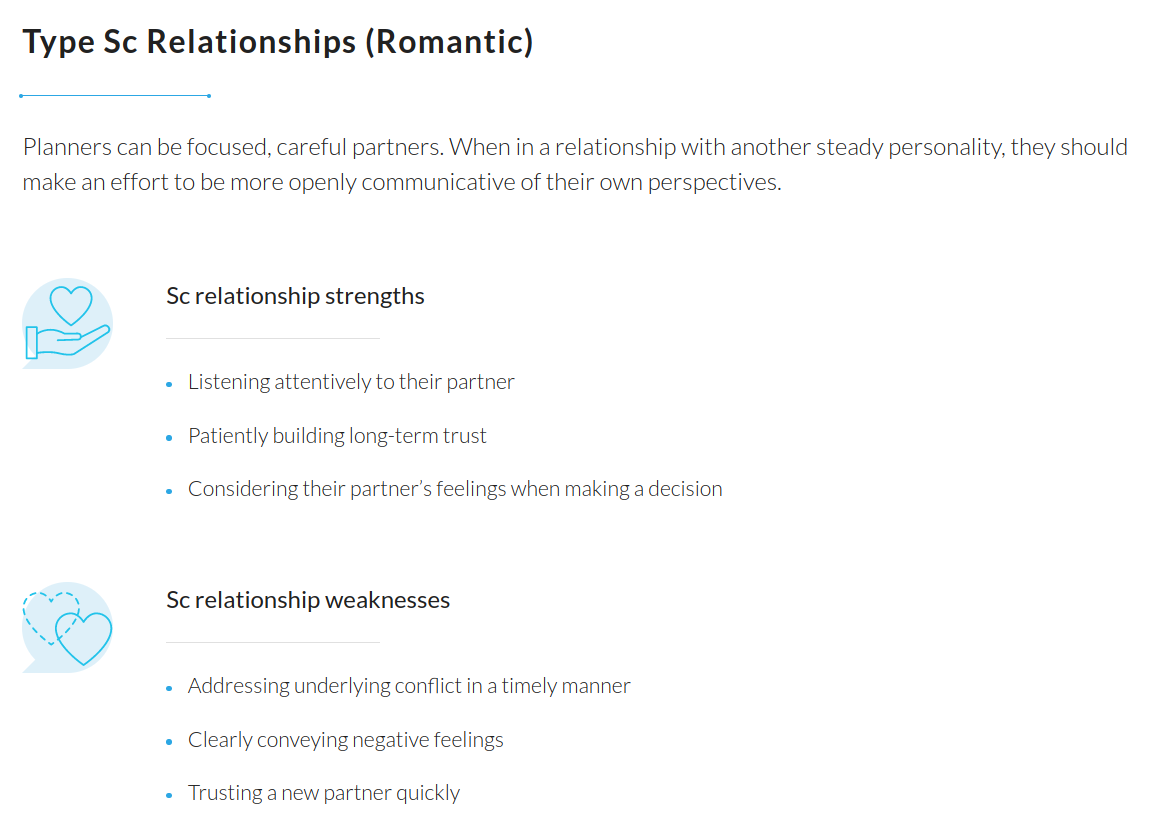
\includegraphics[scale=.275]{images/Sc}
	\end{center}
\end{frame}


\begin{frame}{Tipe SC: Stabilizer}
	\begin{center}
		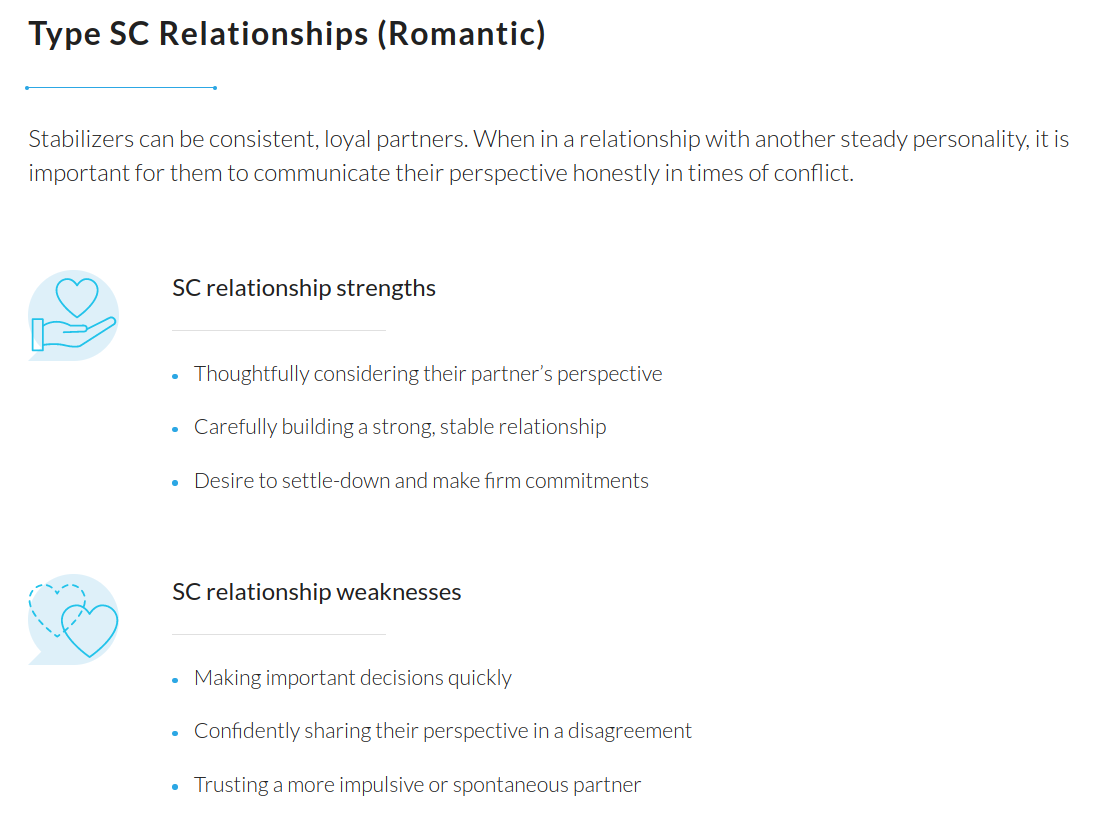
\includegraphics[scale=.275]{images/SC}
	\end{center}
\end{frame}


\begin{frame}{Tipe Cs: Editor}
	\begin{center}
		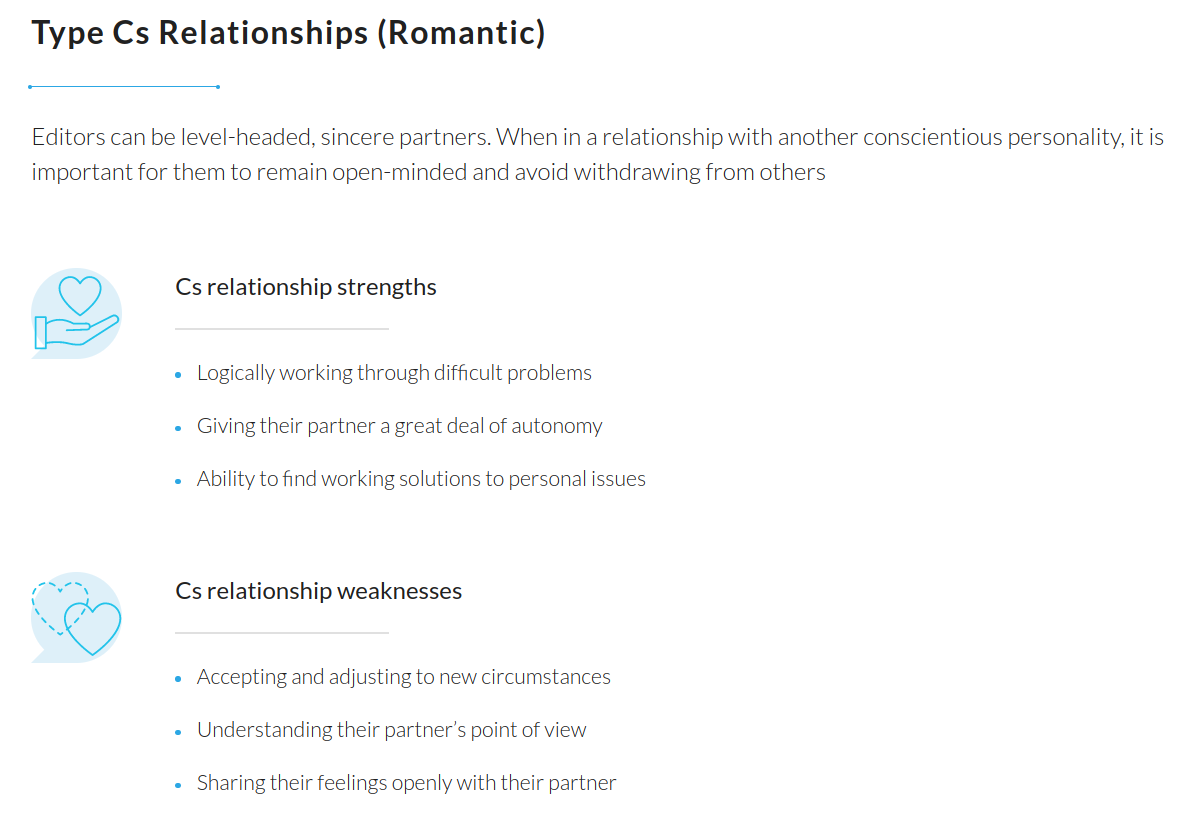
\includegraphics[scale=.275]{images/Cs}
	\end{center}
\end{frame}


\begin{frame}{Tipe C: Analyst}
	\begin{center}
		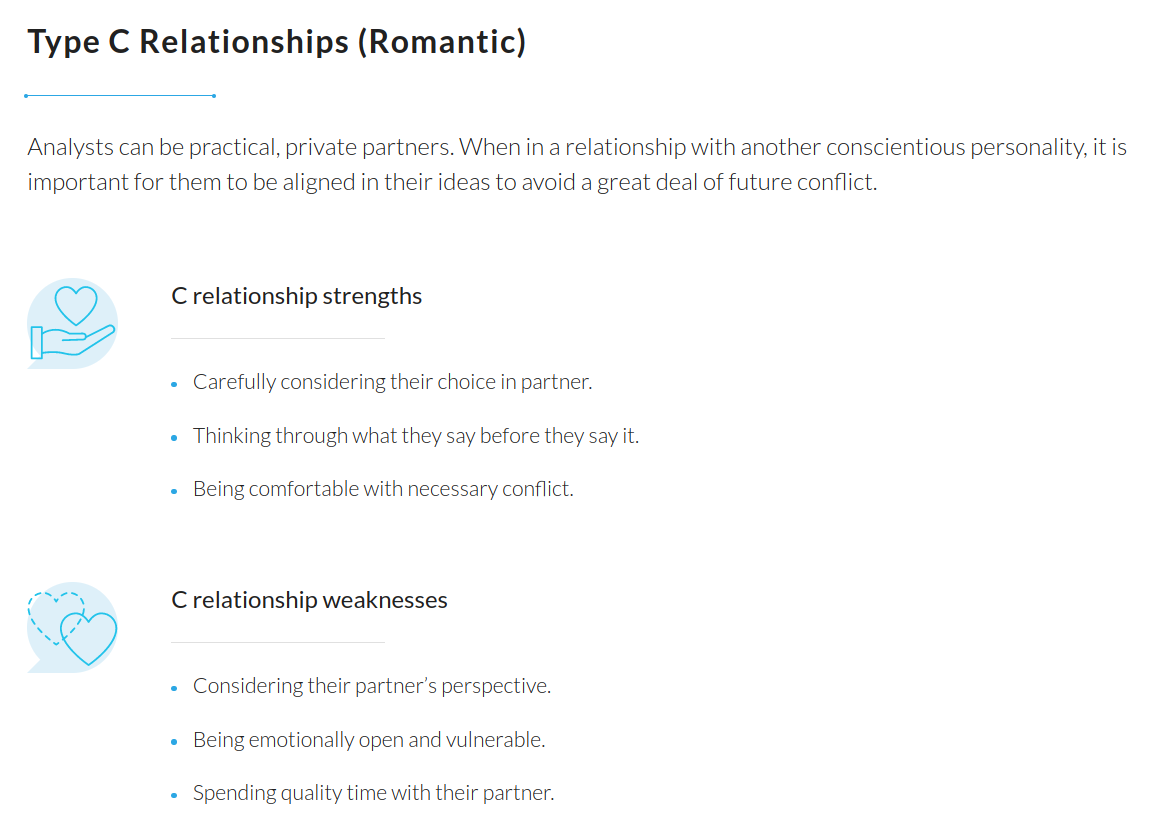
\includegraphics[scale=.275]{images/C}
	\end{center}
\end{frame}

\begin{frame}{Tipe CD: Questioner}
	\begin{center}
		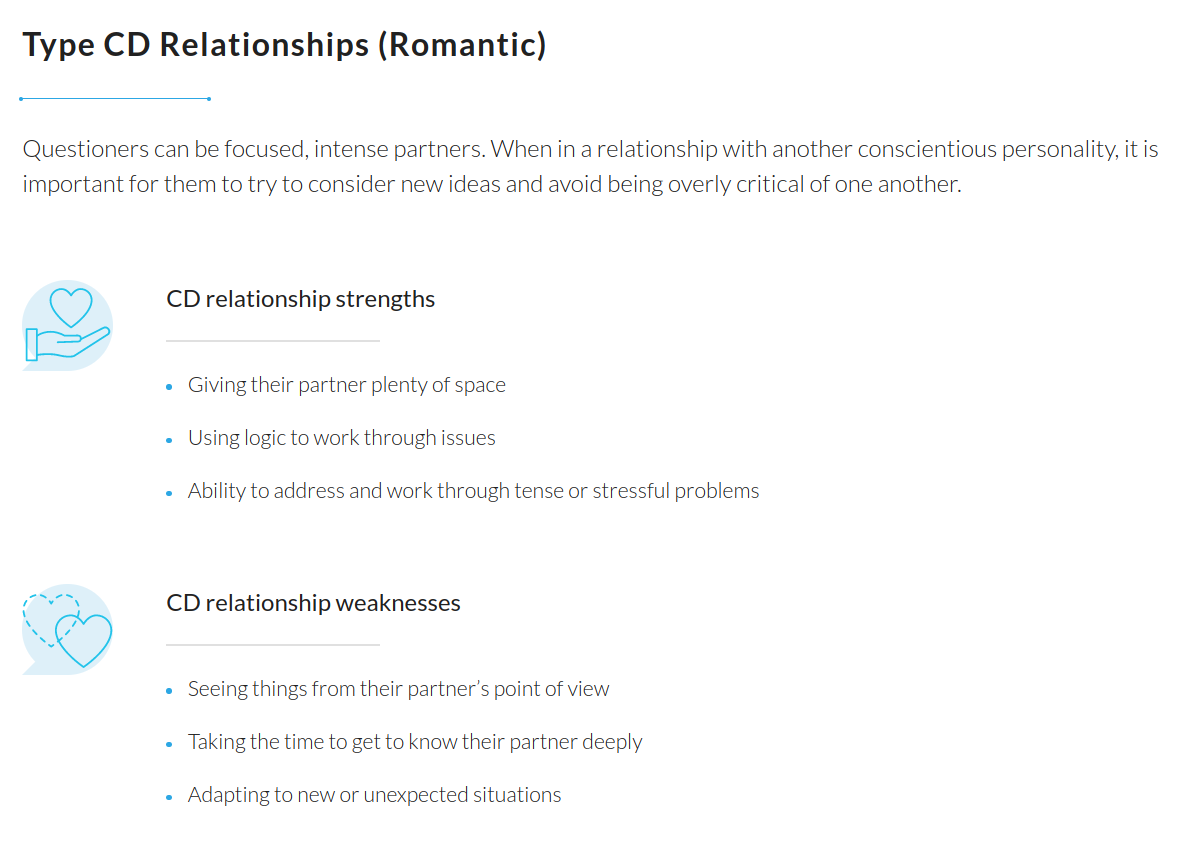
\includegraphics[scale=.275]{images/CD}
	\end{center}
\end{frame}

\begin{frame}{Tipe Dc: Architect}
	\begin{center}
		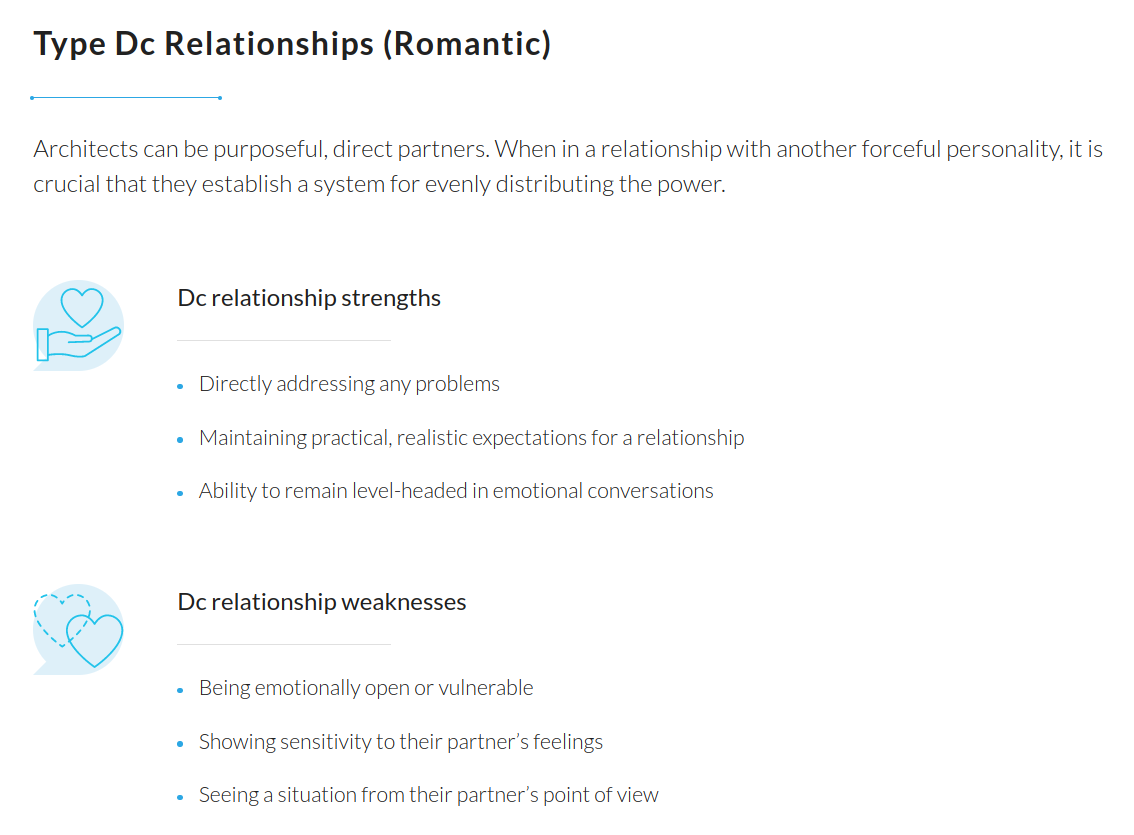
\includegraphics[scale=.275]{images/Dc}
	\end{center}
\end{frame}



%\begin{frame}{Blocks}
%\begin{block}{Block Title}
%You can also highlight sections of your presentation in a block, with it's own title
%\end{block}
%\begin{theorem}
%There are separate environments for theorems, examples, definitions and proofs.
%\end{theorem}
%\begin{example}
%Here is an example of an example block.
%\end{example}
%\end{frame}


% All of the following is optional and typically not needed. 
%\appendix
%\section<presentation>*{\appendixname}
%\subsection<presentation>*{For Further Reading}
%
\begin{frame}[allowframebreaks]
  \frametitle<presentation>{Referensi}
    {\footnotesize
    \bibliographystyle{apalike}
    \bibliography{references}
    }    
\end{frame}

%\makeatletter % to change template
%    \setbeamertemplate{headline}[default] % not mandatory, but I though it was better to set it blank
%    \def\beamer@entrycode{\vspace*{-\headheight}} % here is the part we are interested in :)
%\makeatother

%\begin{frame}[plain]
%		\centering
\includegraphics[scale=0.5]{Logo-Maranatha-Untuk-Belakang-02}	
%\end{frame}

\begin{frame}[plain]
		\centering
\includegraphics[scale=1]{images/thank-you}	
		hendra.bunyamin@it.maranatha.edu
\end{frame}

\end{document}

